% ch19: 微分中值定理
\chapter{微分中值定理——罗尔、拉格朗日、柯西}
\begin{applicationbox}
学完本章：掌握三个中值定理及其关系，会用中值定理证明不等式
\end{applicationbox}

\section{罗尔定理}
若 \(f\) 在 \([a,b]\) 连续、\((a,b)\) 可导、且 \(f(a)=f(b)\)，则存在 \(c\in(a,b)\) 使 \(f'(c)=0\)。

\textbf{ε-δ 证明：} 若 \(f\) 在 \([a,b]\) 上恒为常数，则任意 \(c\) 处 \(f'(c)=0\)，结论成立。
否则 \(f\) 在内部某点取到最大值或最小值（由闭区间上连续函数的最值定理）。
设 \(c\) 为极值点，不妨设是最大值点。取 \(h\) 充分小使 \(c+h\in(a,b)\)，
则 \(f(c+h)\le f(c)\)。当 \(h>0\) 时 \(\frac{f(c+h)-f(c)}{h}\le0\)；
当 \(h<0\) 时 \(\frac{f(c+h)-f(c)}{h}\ge0\)。
令 \(h\to0\) 取极限，由导数存在得 \(f'(c)=\lim_{h\to0^+}\le0\) 且 \(f'(c)=\lim_{h\to0^-}\ge0\)，
故 \(f'(c)=0\)。\quad\(\blacksquare\)

\section{拉格朗日中值定理}
若 \(f\) 在 \([a,b]\) 连续、\((a,b)\) 可导，则存在 \(c\in(a,b)\) 使：
\[f'(c) = \frac{f(b)-f(a)}{b-a}\]

\textbf{ε-δ 证明：} 构造辅助函数
\[
g(x)=f(x)-\frac{f(b)-f(a)}{b-a}(x-a)
\]
则 \(g(a)=f(a)\)，\(g(b)=f(b)-\frac{f(b)-f(a)}{b-a}(b-a)=f(a)\)，即 \(g(a)=g(b)\)。
由罗尔定理，存在 \(c\in(a,b)\) 使 \(g'(c)=0\)。
而 \(g'(x)=f'(x)-\frac{f(b)-f(a)}{b-a}\)，故 \(f'(c)=\frac{f(b)-f(a)}{b-a}\)。\(\blacksquare\)

\begin{center}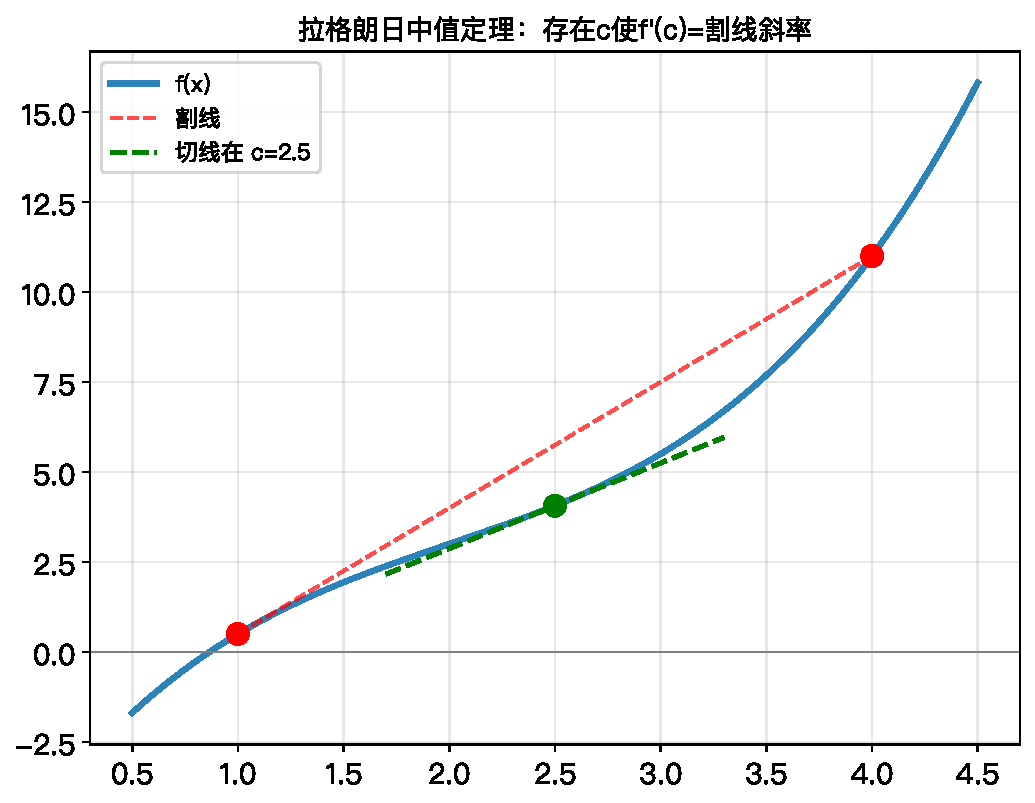
\includegraphics[width=0.6\textwidth]{figures/ch19_mvt.pdf}\end{center}

\begin{examplebox}[1]
证明 \(|\sin b - \sin a| \le |b-a|\)。由中值定理，\(\sin b-\sin a = \cos c \cdot (b-a)\)，\(|\cos c|\le1\)。
\end{examplebox}

\section{柯西中值定理}
若 \(f,g\) 在 \([a,b]\) 连续、\((a,b)\) 可导且 \(g'(x)\neq0\)，则存在 \(c\in(a,b)\) 使：
\[\frac{f(b)-f(a)}{g(b)-g(a)} = \frac{f'(c)}{g'(c)}\]

\section{习题}
\begin{exercise}[0] 罗尔定理要求 \(f(a)\) 和 \(f(b)\) 有什么关系？\end{exercise}
\begin{exercise}[0] 拉格朗日中值定理的几何意义是什么？\end{exercise}
\begin{exercise}[0] 中值定理中的 \(c\) 在哪个区间内？\end{exercise}
\begin{exercise}[0] 若 \(f'(x)=0\) 恒成立，\(f(x)\) 是什么函数？\end{exercise}
\begin{exercise}[1] 验证 \(f(x)=x^2-4x+3\) 在 \([1,3]\) 上满足罗尔定理条件，求 \(c\)。\end{exercise}
\begin{exercise}[1] 对 \(f(x)=x^2\) 在 \([1,3]\) 上应用中值定理求 \(c\)。\end{exercise}
\begin{exercise}[1] 证明 \(\sqrt{1+h} < 1 + h/2\)（\(h>0\)）。\end{exercise}
\begin{exercise}[1] 若 \(f'(x)=2\)，且 \(f(1)=3\)，求 \(f(x)\)。\end{exercise}
\begin{exercise}[2] 验证 \(f(x)=x^3-3x\) 在 \([-\sqrt{3},\sqrt{3}]\) 上满足罗尔定理。\end{exercise}
\begin{exercise}[2] 证明 \(|\arctan b - \arctan a| \le |b-a|\)。\end{exercise}
\begin{exercise}[2] 用中值定理证明 \(e^x > 1+x\)（\(x>0\)）。\end{exercise}
\begin{exercise}[2] 若 \(f'(x)=3x^2\)，\(f(0)=1\)，求 \(f(x)\)。\end{exercise}
\begin{exercise}[3] 证明 \(\frac{b-a}{b} < \ln\frac{b}{a} < \frac{b-a}{a}\)（\(0<a<b\)）。\end{exercise}
\begin{exercise}[3] 证明 \(|\sin x - \sin y| \le |x-y|\)。\end{exercise}
\begin{exercise}[3] 用中值定理证明 \(\ln(1+x) < x\)（\(x>0\)）。\end{exercise}
\begin{exercise}[3] 若 \(f'(x)=g'(x)\) 对所有 \(x\) 成立，证明 \(f(x)=g(x)+C\)。\end{exercise}
\begin{exercise}[3] 证明 \(x > \sin x > x - x^3/6\)（\(x>0\)）。\end{exercise}
\begin{exercise}[4] 若 \(f''(x)>0\)，证明 \(f\) 是凸函数。\end{exercise}
\begin{exercise}[4] 证明方程 \(x^3-3x+1=0\) 在 \((0,1)\) 内至多有一个根。\end{exercise}
\begin{exercise}[4] 用中值定理证明 \(\sqrt{1+x} < 1 + x/2\)（\(x>0\)）。\end{exercise}
\begin{exercise}[4] 证明若 \(f'(x)=f(x)\)，则 \(f(x)=Ce^x\)。\end{exercise}
\begin{exercise}[4] 证明 \(\lim_{x\to0} \frac{\sin x}{x}=1\) 用中值定理。\end{exercise}
\begin{exercise}[5] 证明 \(\frac{x}{1+x^2} < \arctan x < x\)（\(x>0\)）。\end{exercise}
\begin{exercise}[5] 若 \(f\) 在 \([0,1]\) 可导，\(f(0)=0\)，\(f(1)=1\)，证明存在 \(c\) 使 \(f'(c)=1\)。\end{exercise}
\begin{exercise}[5] 证明：若 \(f'(x)\) 有界，则 \(f\) 一致连续。\end{exercise}
\begin{exercise}[5] \(f\) 在 \([0,1]\) 可导，\(f(0)=0\)，\(f(1)=1\)，证明存在不同 \(a,b\) 使 \(1/f'(a)+1/f'(b)=2\)。\end{exercise}
\begin{exercise}[6] 证明达布定理：导函数具有介值性。\end{exercise}
\begin{exercise}[6] 若 \(f\) 在 \([a,b]\) 可导且 \(f'(a)<k<f'(b)\)，证明存在 \(c\) 使 \(f'(c)=k\)。\end{exercise}
\begin{exercise}[6] 证明：若 \(f\) 在 \(\mathbb{R}\) 上可导且 \(|f'(x)|\le M\)，则 \(f\) 一致连续。\end{exercise}
\begin{exercise}[7] 设 \(f\) 在 \([0,1]\) 可导，\(f(0)=0\)，\(f(1)=1\)，\(f'(x)\neq0\)，证明存在 \(c,d\) 使 \(1/f'(c)+1/f'(d)=2\)。\end{exercise}
